\section{Introduction}
\label{sec:intro}

\paragraph{Motivation}
Programming systems that interact with physical processes are gaining importance for robotics, manufacturing, IoT, and other cyber-physical systems. Traditional domain specific languages and models for these systems are platform specific as they combine various low-level sensing, communication, and control tasks with the higher-level applications~\cite{nordmann2014robotics}. For sophisticated high-level software applications, the tight-coupling of application design with platform-specific details hinders development, portability, code reuse,  verification, and synthesis.

This need for raising the level of abstraction and separating the \emph{platform-independent} decision and coordination tasks from \emph{platform-dependent} concerns such as sensing, communication, and low-level control motivates our work. For example, to develop an application for distributed package delivery with mobile robots in a building, the code for assigning robots to visit way-points in different rooms, load-balancing, and handling failures.  This application design is independent of the underlying platform, and therefore, should ideally be transferable across platforms. In contrast, steering control of the individual vehicles, indoor positioning, and message-level communication protocols are tied to the specific hardware.

Developing the above type of application is becoming important and at the same time the task remains arduous with current  programming tools. The developer will have to keep track of communication between different sensors, actuators, and program variables. ROS~\cite{rosbridge_suite,ros} provides publish-subscribe libraries and low-level messaging standards, but the semantics of these schemes are not integrated with any high-level programming abstractions. Similarly, coordination across multiple robots has to be built from the ground up. In order to simulate and test the application, one has to create different threads or instances for the developed code corresponding to different agents, and in addition the agent programs have to be harnessed in a physical world simulator with proper sensor and actuator models. In order to analyze correctness, one has to first define the semantics of the system. This  is again challenging  as this distributed cyber-physical systems has multi-scale data flow across different components. A further concern is the gap between the system being analyzed and the artifact that is actually executing. 

An ongoing project at our University aims to address  these challenges by designing, developing, and evaluating a programming system for distributed robotics. \footnote{Information about this project and the links to downloadable software will be made available to the reviewers upon request. We omit the information here for the sake of maintaining anonymity.} In this paper, we present the design and the implementation of the  {\em Koord langauge} and its supporting software tools which is the  central piece in this programming system.


%
%\begin{figure}[h!]
%\centering
%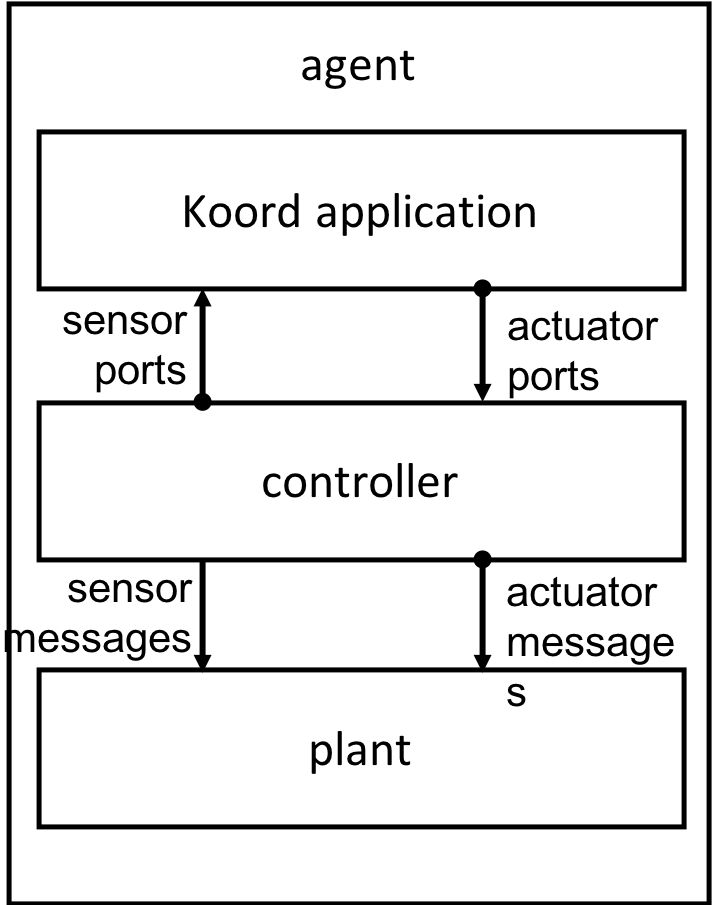
\includegraphics[width=0.48\textwidth]{figs/arch.png}
%\caption{\small CyPhyHouse framework. Major tools shown in blue.}
%\label{fig:arch}
%\end{figure}
%
\subsection{Contributions}
\subsubsection{Design and implementation of $\lgname$ language}
{\em We present a clean-slate design and implementation of an event-driven programming language, for distributed cyber-physical systems, namely $\lgname$.} 
%
$\lgname$ combines distributed shared memory abstraction for coordination across agents and a synchronous model of communication with the physical environment through sensors and actuators, in a familiar precondition-effect style language.
%

Consider the simple line-formation program in which a set of $N$ robots form a equi-spaced line starting from arbitrary positions. The elementary algorithm is for each robot $i$ to repeatedly move towards the midpoint of the line joining the positions of $i-1$ and $i+1$. The extremal robots with ids $0$ and $N-1$ stay fixed. This is a archetypal protocol for synchronization, pattern formation, and consensus~\cite{Tsitsiklis:1986,Blondel,Magnusbook2010,faxmurray} in distributed robotics.
%

The $10$ line long  $\lgname$ program implementing this algorithm is shown below. Among these $10$ lines, lines 1-5 import the {\em controller module\/} called {\em Motion\/} that enables this program to access the sensor port with the agent's position $(\mathit{psn})$ and the actuator port $(\mathit{target})$. Another powerful feature of $\lgname$ used in this program is the single-write multi-reader ({\bf allread}) shared array $x$, in which component $x[i]$ records the position of the $i^{th}$ robot in each round. 
%
The one and only event in this program $\mathit{TargetUpdate}$ (lines 5-9) is quite simple: it updates the target position of the agent  to be the midpoint of its neighbors. The shared variable makes this program easy to read and remarkably close to the textbook version of the line-formation algorithm. Figure~\ref{fig:shapeformplots} shows the result of simulating (a slightly modified) version of $\mathit{Lineform}$ on the $\lgname$ simulator with $25$ robots forming a 3D-shape. The $\lgname$ compiler can also generate executables that can be deployed on several mobile robotic hardware platforms. We mention these capabilities briefly in Section~\ref{sec:intro:hardwaretc}, however, the complete details will be presented in a future publication. 
 

% \belowcaptionskip=-10pt
\begin{lstlisting}[label=lineform,caption=Lineform $\lgname$ program]
   using Motion:
      sensors pos psn
      actuators target
   allread: pos x $\label{lineformp}$
   TargetUpdate:
      pre True
      eff if not(pid == $\NMAX$ - 1 or pid == 0):
         Motion.target = mid(<x[pid+1],x[pid-1]>)
         x[pid] = Motion.psn
\end{lstlisting}

%\renewcommand{\lstinputlisting}[1][]{\oldlstinputlisting[frame=lines,#1]}
 
%\begin{figure}[ht!]
%	\label{fig:lineform}
%	\noindent
%	\begin{center}
%		\scriptsize
%		\two{0.4}{0.6}
%		{\lstinputlisting[language=xyzNums,frame=lines]{code/lineform.tex}}
%	\par        
%	\end{center}
%	\caption{\small $\lgname$ program for line formation ({\em Left}) and its mathematical counterpart in robotics and control textbooks ({\em Right}).}
%\end{figure}

%The shared \emph{allread} variable $p$ (Line\ref{lineformp}) is used by the agents to communicate their position to the other robots. The function \emph{midpoint} is a part of the library functions provided for the data type \emph{pos}; where $$\mathit{midpoint}(p_1,p_2,\ldots,p_n) = pos(\frac{\Sigma_n p_i.x}{n},\frac{\Sigma_n p_i.y}{n},\frac{\Sigma_n p_i.z}{n}) $$.
%

%We have implemented a compiler for $\lgname$ that generates executable Python programs that can be either simulated in a discrete event simulator (discussed below) or 

\subsubsection{\K semantics for $\lgname$}
% motivation
Implementation of programming languages usually have many bugs. One common source of bug is the gap between the formal semantics of the language and the its implementation as embodied in a compiler. The \K framework~\cite{} closes this gap by \sayan{fill in..}. \sayan{Two senteces introducing K .How and why it works. 2 sentences describing the impact of K.}

We have \sayan{developed ...}
This involved ... 

Our \K implementation of $\lgname$ enables us to ... 

Verification.

\subsubsection{Simulator and applications}

Challenges: 

Discrete event .. threads, motion. 

What it enables. 

\begin{figure}[h!]
\begin{minipage}{0.5\textwidth}
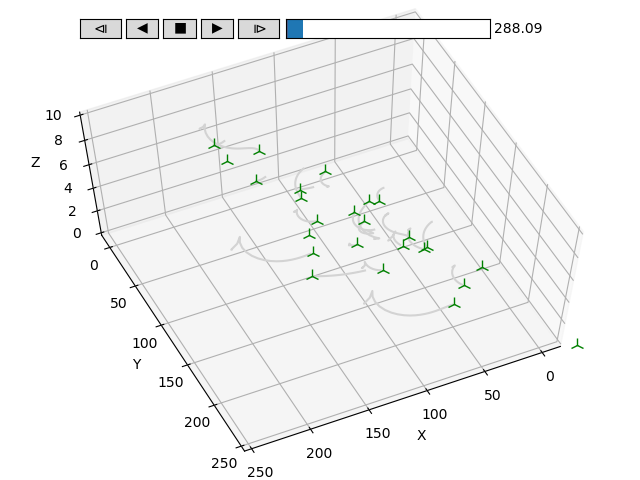
\includegraphics[width=.5\textwidth]{figs/formation1.png}\hfill
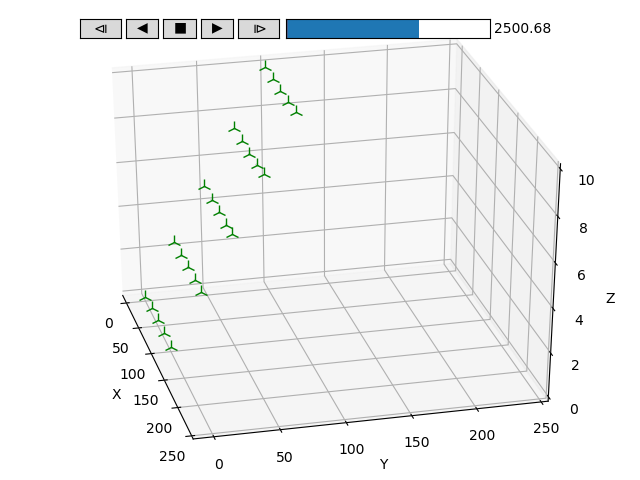
\includegraphics[width=.5\textwidth]{figs/formation5.png}\hfill%
%\includegraphics[width=.3\textwidth]{figs/Platooning_2.png}}\hfill%
\end{minipage}%
\caption{$x$ vs $y$ vs $z$ plots for shapeform. The grey trails represent the positions of the agents in the last 150 time steps.}
\label{fig:shapeformplots}
\end{figure}


\subsubsection{Other by-producsts}


Design and development of the CyPhyHouse open source software system. This includes a discrete event simulator for distributed robotic systems, the application launcher, the run-time logging and monitoring system, and an integrated indoor positioning system. All of these software tools are integrated with our new robot programming language called $\lgname$ and its compiler. 

 First demonstration of the feasibility of end-to-end high-level application development and deployment on a distributed, heterogeneous, platform involving quadcopters and ground vehicles. 

 Demonstration of the feasibility of system-level verification of applications written in $\lgname$. 

Design and development of the $\lgname$ programming language and the supporting $\mathbb{K}$-based~\cite{Kpaper} verification tool \kbmc\, are discussed here for the sake of completeness; those details will appear elsewhere~\cite{koordreport}.

%Design and development of the Koord programming language and the supporting verification tool KoordBMC~\cite{koordreport}--- significant, related but separate efforts---are not contributions of the current paper; we discuss their usage for the sake of completeness. 
% completely describing the framework. 
% the Demonstration of an example application development using CyPhyHouse tools and deployment on a physical system using multiple quadcopters.
%Non-contributions: Spell these out  to avoid misdirected criticisms and conflict with overlapping publications.
%\begin{itemize} 
%\item Language design
%\item Verification tools.
%\item Low-level controller design for vehicles.
%\end{itemize} 

%\begin{figure}[h!]
%\centering
%\includegraphics[width=0.45\textwidth]{figs/exp_traces.png}
%\caption{\small Experimental run in our testbed. The traces show the path of each robot for the last $2$ seconds. }
%\label{fig:exp_traces}
%\end{figure}


\footnote{\href{https://cyphyhouse.github.io/index.html}{https://cyphyhouse.github.io}}: an open source software framework for programming, rapid deployment, and testing of distributed robotics applications. 
\sayan{The high-level $\lgname$ language enables users to write succinct distributed coordination applications without getting bogged down by messaging and thread management issues (See Examples in \reffig{lineform} and \reffig{taskapp}).}
Using the CyPhyHouse framework around $\lgname$, a user can code, compile, launch, and run applications in a highly-automated fashion (\reffig{arch}). 
\sayan{The framework has been built over three years and has more than 100k lines of source code.}


    - problems in the space of (distributed) CPS, robotics, automation .
    - Coordination and Control issues. 
    - why we need something like Koord /why something like koord helps computer scientists (non roboticists) work with robotics. 
    - what is koord and how Koord specifically accommodates users
    - how we built koord. 
    - what is this paper
    - Related work
    
    \section{Related work}
    \label{sec:related}
    \sayan{Modern programming languages like C\# and Swift, and   compiler infrastructures like LLVM~\cite{llvm} have revolutionized the application development ecosystem in mobile computing.
%\paragraph*{D.} 
Inspired by these successes, there is a surge of interest in open and portable languages that raise the level of abstraction~\cite{Buzzlanguage,Bohrer:2018:VVC:3192366.3192406,reactlang,williams2003model} (For an earlier survey of Domain Specific Programming Languages (DSLs) for robotic systems see~\cite{Nordmann2014}. Most of these older languages are proprietary or generate executable files that are tied to specific platforms)}. 
%
Buzz~\cite{Buzzlanguage} and React~\cite{reactlang} fall in this category as does our language $\lgname$. 
The Live Robot Programming language~\cite{campusanofabry:lrp2016} not only provides a higher-level programming abstraction in terms of nested state machines, but also allows the program to be changed while running, hence reducing the feedback loop across writing, compiling, and testing of robot programs. 
%The goals of React language for robotics aligns with our goals~\cite{react-lang}
Buzz currently does not  connect with  verification tools, and the verification approach implemented with React uses precise models of the environment and performs model checking using dReal~\cite{Gao2013}. 
In contrast, our environment implementations allow for imprecise models, with a verification approach using sensitivity analysis~\cite{DryVR2017}.
%Our approach is also similar in spirit to the Reactive Model-based Programming Language (RMPL)
%~\cite{williams2003model}.
%
%There is been more recent development of domain specific languages for general cyber-physical systems (CPS)~\cite{pradhan2015chariot}. The main challenge addressed in this line of work is in supporting reconfiguration of complex, heterogeneous software components, for handling failures. 
%
%There has also been work on programming abstractions for coordinating CPS~\cite{distCPSSri,Bundle}. 
%A group-based abstraction that facilitates dynamic creation of logical collections of sensors and actuators is presented in~\cite{Bundle}. 
%
%
%%React reactive robot programming language~\cite{DogmusEP15}.
%% 
The Robotarium project provides remote end-to-end access to a  multi-robot research facility, but not languages and development tools~\cite{robotarium}. 
The  VeriPhy project~\cite{Bohrer:2018:VVC:3192366.3192406} shares a similar goal to CyPhyHouse; however, instead of a programming language, the starting point is differential dynamic logic~\cite{Bohrer:2017:FVD:3018610.3018616},  and there are significant differences  in the underlying verification engines used (KeYmaera X, HOL instead of K, Z3, DryVR).
%

``Correct-by-construction'' synthesis from high-level temporal logic specifications has been applied to mobile robotic systems (see, for example~\cite{kress2009temporal,kloetzer2008fully,wongpiromsarn2010receding,wongpiromsarn2011tulip,ulusoy2013optimality}).
% Many of these approaches have been applied to mobile robotic systems. 
\sayan{Our point of view on automating robot programming is different in that we expect that the programmer's creativity and efforts will be necessary well beyond writing high-level specs in solving distributed robotics problems; consequently only the tedious and standard steps in coordination and control are automated using the $\lgname$ compiler.}

%. A
%correct-by-construction synthesis algorithm takes as input a high-level requirement (for example, ``from room A to B and see if you find a chair'') to generate robot programs for accomplishing
%this task. In our approach, 

%\paragraph*{Languages for distributed shared memory systems}
%
Programming systems using the  shared memory paradigm have been developed for several distributed computing systems~\cite{dsm1991,Adve96sharedmemory,Azure,Cassandra,Dynamo}.
Specifically, P~\cite{Planguage}  and PSync~\cite{PSyncLanguage} are DSLs for  asynchronous partially  distributed systems, but cyber-physical interactions are not supported. 
%DSM has also been proposed as a programming model in the context of wireless networks~\cite{hcs,rs}. 
%These  programming models are defined mathematically in terms of state machines or in terms of APIs, and are  typically not embodied in a programming language with carefully designed syntax and semantics to enforce the models. 
$\lgname$  provides a distributed shared variable abstraction for coordinating multiple agents. 
%\sayan{This enables users to write succinct, textbook-like programs without struggling with messy code for message handling and thread management}. 
The consistency semantics implemented here are that the writes to shared variables are propagated to all the agents, and become visible to other agents reading the variable after one round ($\delta$ time units).
In the fault-free synchronous model considered here a gossip algorithm-based is used to implement this semantics in the $\lgname$ runtime system. 
% The framework of~\cite{Hotline_CPS_srivastava} supports shared memory over multi-hop wireless networks, with a consistency model analogous to {\em release} consistency.  
%

%
%\paragraph*{Uncertainty and Robotics Abstractions}
%$\lambda_O$~\cite{park2005probabilistic} is a probabilistic programming language in which sampling methods are used to specify probability distributions, while expressing and reasoning about these methods formally. It finds application in robot localization and mapping. In the same vein, $\mathit{Uncertain}\langle T\rangle$~\cite{bornholt2014uncertain} provides a programming language abstraction for uncertain data. It is a departure from previous probabilistic programming languages in the wide range of developers it serves, as opposed to being accessible only by experts. The language provides abstractions and semantics for uncertain data, like sensed information about location, temperature, etc. While $\lgname$ does not currently perform reasoning involving uncertainty in sensor readings or agent localization currently, these are realistic concerns that can be explored by exploiting the extensibility of the $\lgname$ semantics implemented in \K. While these languages provide semantics for uncertainity in robot abstractions and sensing issues, they do not provide distributed application design capabilities. 
%\sayan{I did not find much about this. Formal verification of mobile robot protocols: the DVE language, which is the input format of the model-checkers DiVinE and ITS tools, and formally prove the equivalence of the two models.}
%\item  
%Buzz, a novel programming language for heterogeneous robot 
%swarms. Buzz advocates a compositional approach, offering primitives to define swarm 
%behaviors both from the perspective of the single robot and of the overall swarm. 
%
%\item 

%Voltron programming system to explore the concept of team-level programming in active sensing applications. Voltron offers programming constructs to create the illusion of a simple sequential execution model while still maximizing opportunities to dynamically re-task the drones as needed. We implement Voltron by targeting a popular aerial drone platform, and evaluate the resulting system using a combination of real deployments, user studies, and emulation. Our results indicate that Voltron enables simpler code and produces marginal overhead in terms of CPU, memory, and network utilization. In addition, it greatly facilitates implementing correct and complete collaborative drone applications, compared to existing drone programming systems. (?) 
%\end{enumerate}

